\documentclass{article}
\usepackage{graphicx} % Para incluir imágenes
\usepackage[spanish]{babel}
\usepackage{makeidx}
\usepackage{geometry}
\usepackage{graphicx}
\usepackage{caption}
\usepackage{pdfpages}



\geometry{a4paper, total={170mm,257mm}, left=20mm, top=20mm}
\renewcommand{\familydefault}{\sfdefault}


\begin{document}
\begin{titlepage}
    \centering
    \Large
    Universidad Central de Venezuela\\
    Facultad de Ingeniería\\
    Escuela de Ingeniería Eléctrica
    \vspace*{8cm}

    \Huge
    \textbf{Prelaboratorio Nº 4:} 

    \textbf{Respuesta en frecuencia}
    \vfill


    \Large

    Emerson Warhman \\
    C.I. 25.795.480 \\
    \today

\end{titlepage}
\tableofcontents
\newpage

\section{Introducción}

Los amplificadores operacionales (op-amps) son dispositivos versátiles que encuentran aplicaciones tanto en circuitos lineales como no lineales. Mientras que en configuraciones lineales se utilizan principalmente para operaciones de amplificación y filtrado, sus aplicaciones no lineales abren un panorama de posibilidades en generación y conformación de señales. Este informe explora tres configuraciones fundamentales de op-amps en régimen no lineal: el oscilador de puente de Wien, los multivibradores (astable y monoestable) y los generadores de funciones.

El \textbf{oscilador de puente de Wien} representa una aplicación clásica en generación de señales sinusoidales. Su diseño aprovecha el balance entre una red de realimentación positiva (para mantener las oscilaciones) y un mecanismo de control de amplitud (usualmente mediante diodos o JFETs) que garantiza estabilidad en la señal de salida. La frecuencia de oscilación está determinada por la relación $f_o = \frac{1}{2\pi RC}$, demostrando cómo componentes pasivos simples pueden definir características fundamentales de la señal generada.

Los \textbf{multivibradores} ilustran la capacidad de los op-amps para trabajar en conmutación:
\begin{itemize}
    \item El \textbf{astable} opera como oscilador libre, generando una onda cuadrada continua cuya frecuencia depende de los elementos RC en el circuito
    \item El \textbf{monoestable} produce un pulso de duración fija ante un disparo externo, siendo útil en aplicaciones de temporización
\end{itemize}

Los \textbf{generadores de funciones} amplían estas capacidades para producir formas de onda complejas (triangulares, diente de sierra, etc.), a menudo mediante la integración controlada de señales cuadradas. Estos circuitos encuentran aplicaciones prácticas en sistemas de comunicaciones, instrumentación médica y equipos de prueba electrónicos.

Este estudio experimental permitirá verificar los principios teóricos de operación, analizar las relaciones entre los componentes y los parámetros de salida, y evaluar las limitaciones prácticas de estos circuitos. Particular atención se dedicará al análisis de distorsión armónica en el oscilador Wien y a la precisión temporal en los multivibradores, aspectos críticos para aplicaciones reales.



\section{Resumen}

\section{Marco teorico}

\section{Metodología}

\section{Resultados}

\section{Análisis de resultados}

\section{Conclusiones}

\section{Anexos}
\section{Anexos}

\begin{ilustracion}[ht]
    \centering
    \includegraphics[width=1.0\textwidth]{src/images/p1/p1-hoja-de-datos.jpg}
    \caption{Hoja de datos práctica N° 1}
    \label{ilus:hoja-de-datos-p1}
\end{ilustracion}

\begin{ilustracion}[ht]
    \centering
    \includegraphics[width=1.0\textwidth]{src/images/p2/p2-hoja-de-datos.jpg}
    \caption{Hoja de datos práctica N° 2}
    \label{ilus:hoja-de-datos-p2}
\end{ilustracion}

\begin{ilustracion}[ht]
    \centering
    \includegraphics[width=1.0\textwidth]{src/images/p3/p3-hoja-de-datos.jpg}
    \caption{Hoja de datos práctica N° 3-1}
    \label{ilus:hoja-de-datos-p3-1}
\end{ilustracion}

\begin{ilustracion}[ht]
    \centering
    \includegraphics[width=1.0\textwidth]{src/images/p3/p3-hoja-de-datos-2.jpg}
    \caption{Hoja de datos práctica N° 3-2}
    \label{ilus:hoja-de-datos-p3-2}
\end{ilustracion}

\begin{ilustracion}[ht]
    \centering
    \includegraphics[width=1.0\textwidth]{src/images/p4/p4-hoja-de-datos-1.jpg}
    \caption{Hoja de datos práctica N° 4-1}
    \label{ilus:hoja-de-datos-p4-1}
\end{ilustracion}

\begin{ilustracion}[ht]
    \centering
    \includegraphics[width=1.0\textwidth]{src/images/p4/p4-hoja-de-datos-2.jpg}
    \caption{Hoja de datos práctica N° 4-2}
    \label{ilus:hoja-de-datos-p4-2}
\end{ilustracion}

\begin{ilustracion}[ht]
    \centering
    \includegraphics[width=1.0\textwidth, angle=90]{src/images/p5/p5-hoja-de-datos-1.jpg}
    \caption{Hoja de datos práctica N° 5-1}
    \label{ilus:hoja-de-datos-p5-1}
\end{ilustracion}

\begin{ilustracion}[ht]
    \centering
    \includegraphics[width=1.0\textwidth,angle=90]{src/images/p5/p5-hoja-de-datos-2.jpg}
    \caption{Hoja de datos práctica N° 5-2}
    \label{ilus:hoja-de-datos-p5-2}
\end{ilustracion}

\begin{ilustracion}[ht]
    \centering
    \includegraphics[width=1.0\textwidth, angle=90]{src/images/p5/p5-hoja-de-datos-3.jpg}
    \caption{Hoja de datos práctica N° 5-3}
    \label{ilus:hoja-de-datos-p5-3}
\end{ilustracion}

\includepdf[page=-, width=0.9\textwidth]{src/assets/BC237.pdf}
\captionof{ilustracion}{Hoja de datos del transistor BC237}

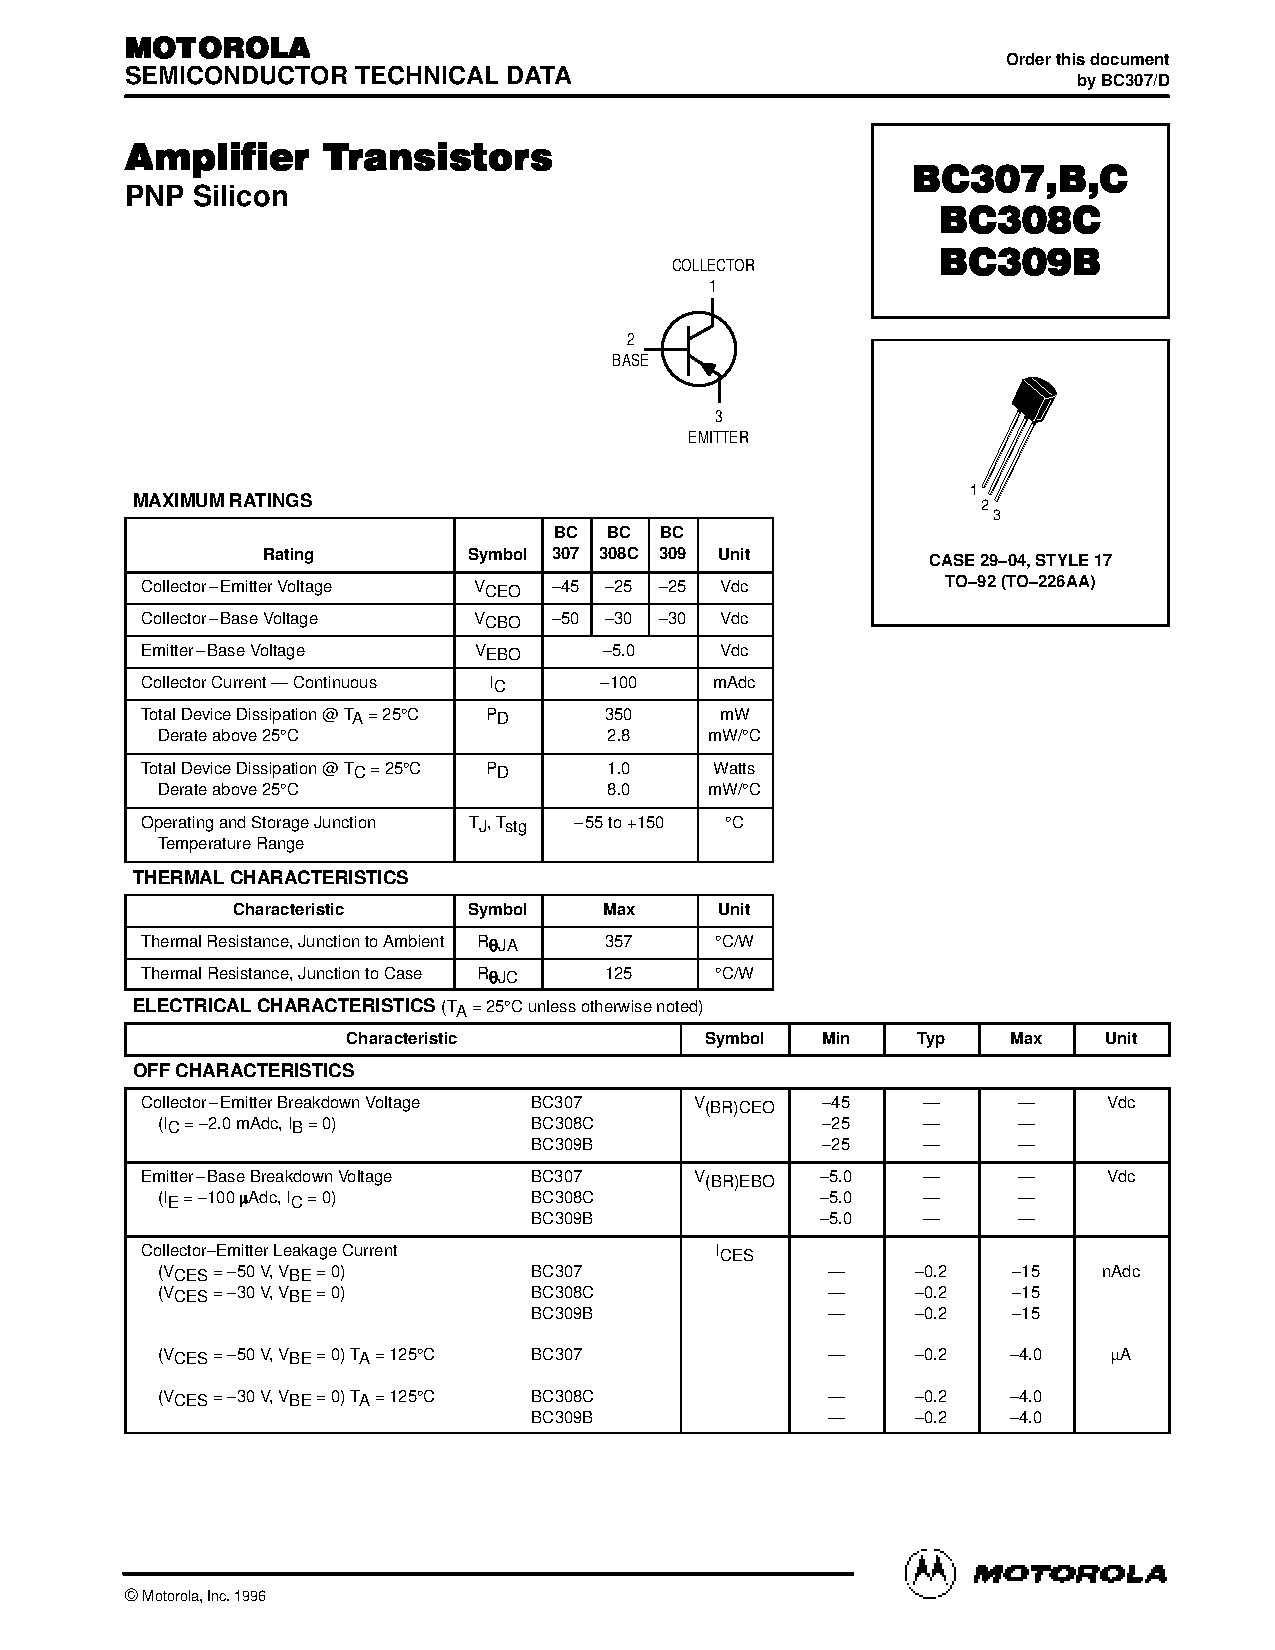
\includepdf[page=-, width=0.9\textwidth]{src/assets/bc307.pdf}
\captionof{ilustracion}{Hoja de datos del transistor BC307}


\end{document}
